\documentclass[a4paper,UTF8]{article}
\usepackage{ctex}
\usepackage[margin=1.25in]{geometry}
\usepackage{color}
\usepackage{graphicx}
\usepackage{amssymb}
\usepackage{amsmath}
\usepackage{amsthm}
%\usepackage[thmmarks, amsmath, thref]{ntheorem}
\theoremstyle{definition}
\newtheorem*{solution}{Solution}
\newtheorem*{prove}{Proof}

\usepackage{float}
\usepackage{multirow}
\usepackage{url}
\usepackage[colorlinks,urlcolor=blue]{hyperref}
\usepackage{enumerate}
\renewcommand\refname{参考文献}


%--

%--
\begin{document}
\title{\textbf{《计算机图形学》3月报告}}
\author{171860509,丁保荣,\href{mailto:1770048119@qq.com}{1770048119@qq.com}}
\maketitle

\tableofcontents

\newpage

\section{综述}
我开发了一款名为Painter的画图工具,它既可以支持命令行模式(用户给定一个指令文件,程序按照指令绘制图形并输出到指定文件),也支持图形界面模式(给用户提供一个user-friendly的界面,供用户进行创作)。

本工具的主要开发语言为Python,图形界面部分主要使用PyQt5库。

本工具提供macOS平台版本,用pyinstaller进行打包,包含了所有的依赖,不需要用户自行安装Python环境或PyQt环境。该版本在macOS 10.15.3下运行正常。

下面主要介绍一下实现过程中遇到的一些算法,还有一些功能的实现与展示。


\section{算法介绍}

\subsection{直线DDA算法}
DDA的算法思想很简单,假设我们有两个点$A(x_0, y_0)$ 和 $B(x_1, y_1)$, 然后我们可以计算两点间的差值$\Delta x  = x_1 - x_0$, $\Delta y = y_1 - y_0$, 不然假设 $abs(\Delta x) > abs(\Delta y)$, 那我们就可以从$(x_0, y_0)$开始,$x$每次增加$dx = \Delta x / abs(\Delta x)$, 而$y$ 每次增加$dy = \Delta y / abs(\Delta x)$, 我们可以把$dx$和$dy$计算出来,接下来每次步进的时候只要进行浮点加减运算,而不用进行浮点乘除运算。因为我们是在屏幕上绘制,需要所有的点都是整数,所以我们生成点的时候需要进行四舍五入。

但还需要注意一点的是,为了保证我们程序的鲁棒性,需要对$x_0 = x_1$且$y_0 = y_1$的情况进行特判,不然会出现除0错误。


\subsection{直线Bresenham算法}
但DDA算法仍然有不足,因为它仍然需要进行浮点运算,那我们能不能只通过整数运算来绘制运算呢?其实是可以的,这里就介绍一下Bresenham算法\cite{wiki:Bresenham's_line_algorithm}。

还是有两个点$A(x_0, y_0)$ 和 $B(x_1, y_1)$,我们这里不妨先假设$x_1 > x_0$, $y_1 > y_0$ 且 $(y_1 - y_0) < (x_1 - x_0)$, 即直线的斜率是小于1的。我们引入一个$error$变量来记录我们的$\hat{y}$与真实的$y$的差值。 我们初始化$error = 0, \hat{x} = x_0, \hat{y} = y_0$, 每次$\hat{x}$步进1, $error$递增$\frac{(y_1 - y_0)}{x_1 - x_0}$, 当$error>0.5$的时候就说明真实的$y$更靠近$\hat{y}+1$了,所以我们把$\hat{y}$递增1,并将$error$递减1。 注意到我们这里的$error$仍然是浮点数,但我们可以把它转化为整数,只要把每次递增的量乘以$x_1 - x_0$变成$y_1 - y_0$, 同时0.5变为$(x_1-x_0)/2$就可以了。这样我们就消除了浮点运算。

如果直线斜率大于1,我们该怎么呢,直接把直线关于$y=x$做对称就可以了,即交换$x$和$y$. 如果直线斜率小于0呢,把$\hat{y}$的步进改成$-1$就可以了。 如果$x_0 > x_1$, 我们交换$A$和$B$就可以了。

这里我们仍然要考虑程序的鲁棒性,对$x_0 = x_1$且$y_0 = y_1$的情况进行特判,不然会出现除0错误。


\subsection{多边形绘制算法}
多边形绘制算法就比较简单了,我们只要按照顺序,对相邻的两个点调用我们的绘制线段的算法就可以了,但要注意一点的是我们还需要对第一个点和最后一个点进行连线。

\subsection{椭圆绘制算法(中点圆生成算法)}
我们这里只考虑中心在原点的椭圆,中心不在原点的椭圆只要加一个平移量就可以了。 我们知道这个椭圆是关于$x$轴和$y$轴对称的,所以我们只需要画1/4个椭圆就可以了,剩下的都可以通过对称得到。

我们这里假设椭圆的方程是$\frac{x^2}{a^2} + \frac{y^2}{b^2} = 1$, 也可以写成$F(x, y) = b^2 x^2 + a^2 y^2 - a^2 b^2  = 0$. 我们画第一象限的$1/4$椭圆,从$(0, x)$开始, 每次$x$先递增1,然后根据决策函数来决定$y$是否改变,当$dy >= dx$时,我们要改成$y$每次递减1,然后根据决策函数来决定$x$是否改变。


所以可以看到我们把这个过程分成了两个部分:

第一个部分的初始决策函数值是$d1 = b^2 - a^2 b + \frac{1}{4} a^2$, 然后如果$d1<0$, 决策函数值应该递增$F(x+2, y-0.5) - F(x+1, y-0.5) = 2b^2x + 3b^2$. 如果$d1>0$, 决策函数值应该递增$F(x+2, y-1.5) - F(x+1, y-0.5) = 2b^2x + 3b^2 - 2a^2 y + 2a^2$ 

第二个部分的初始决策函数值是拿第一部分中最后一个点$(x' , y')$来计算的,即$d2 = F(x'+0.5, y'-1)$. 然后如果$d2<0$, 决策函数值应该递增$F(x+1.5, y-2) - F(x+0.5, y-1) = 2b^2x + 2b^2 - 2a^2 y + 3 a^2 $, 如果$d2 >0 $, 决策函数值应该递增$F(x+0.5, y-2) - F(x+0.5, y-1) = -2a^2 y + 3 a^2$


\subsection{Bezier曲线}

$n$阶Bezier曲线的公式是:$P(t) = \sum\limits_{i=0}^{n} P_i B_{i,n}(t), \ 0 \le t \le 1$. 其中$B_{i,n}(t)$是Bernstein基函数,公式为$B_{i,n}(t) = C_n^i (1-t)^{n-i} t^i$.

公式比较难懂,我们来看一个简单的图示:

\begin{figure}[H]
    \centering
    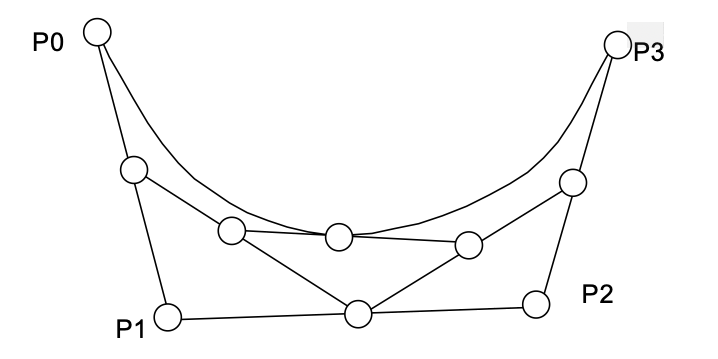
\includegraphics[scale=0.3]{Bezier.png}
\end{figure}

我们采用de Casteljau算法\cite{wiki:De_Casteljau's_algorithm}来绘制Bezier曲线。

我们有$n+1$个点,然后根据这$n+1$个点,在相邻两点之间连线,并在该线段上根据$t$取一点,然后我们得到了$n$个点,一直这么下去,我们能够得到1个点,这个点就是最终Bezier曲线上的点。我们对$t$从0到1进行遍历,就能获得Bezier曲线上的一系列点。

算法的思路差不多就是这样,关于$t$的步长的选取,我现在取的是$0.01$,这个步长的选取也是效果和性能的折中。


\subsection{B样条绘制}
 对于一个有着$n+1$个控制点,$k+1$阶($k$次)B样条曲线,它的公式如下:
    \begin{equation*}
        P(u) = \sum\limits_{i=0}^{n} P_i B_{i, k+1}(u), u \in [u_k, u_{n+1}] 
    \end{equation*}
其中 $B_{i, k+1} (u) = \frac{u - u_i}{u_{i+k} - u_i} B_{i,k}(u) + \frac{u_{i+k+1 - u}}{u_{i+k+1} - u_{i+1}} B_{i+1, k} (u)$. 

关于$B_{i,k}$的Base case是:
    \begin{equation*}
        B_{i, 1} = \begin{cases}
            1, & u \in [u_i, u_{i+1}] \\
            0, & \text{otherwise}
        \end{cases}
    \end{equation*}

    所以我们只要根据这个公式计算每一个点就可以了。

\subsection{平移变换算法}

平移变换就比较简单,我们只需要对图元的所有控制点进行$(dx, dy)$的增量操作就可以了。 即 $(x_0, y_0) \rightarrow (x_0 + dx, y_0 + dy)$


\subsection{旋转变换算法}
旋转变换也比较简单,我们只需要对图元的所有控制点相对于旋转中心做旋转变换就可以了,即乘上了一个旋转变换的矩阵(相对于旋转中心):
    \begin{equation*}
        \begin{bmatrix}
            \cos{\theta} & -\sin{\theta} \\
            \sin{\theta} & \cos{\theta} \\
        \end{bmatrix}
    \end{equation*}

    所以如果$(x_1, y_1)$以$(x_0, y_0)$为中心旋转$\theta$角度的话,首先计算$\Delta x  = x_1 - x_0$, $\Delta y = y_1 - y_0$, 然后旋转后的坐标就是$(\Delta x * \cos{\theta} - \Delta y * \sin{\theta} + x_0 , \Delta x * \sin{\theta} + \Delta y * \cos{\theta} + y_0 )$.


\subsection{缩放变换算法}

缩放变换也不是很难,我们将相对于缩放中心的距离乘以一个系数就行了。

所以如果$(x_1, y_1)$以$(x_0, y_0)$为中心缩放$k$倍的话,首先计算$\Delta x  = x_1 - x_0$, $\Delta y = y_1 - y_0$, 然后缩放后的坐标就是$(\Delta x * k + x_0, \Delta y * k + y_0)$



\subsection{Cohen-Sutherland线段裁剪算法}

Cohen-Sutherland线段裁剪算法\cite{wiki:Cohen–Sutherland_algorithm}可以用一个简单的图示来阐述:

\begin{figure}[H]
    \centering
    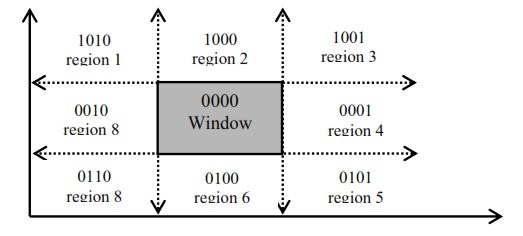
\includegraphics[scale=1.0]{clip1.jpg}
\end{figure}

我们把二维平面分割成九个部分,按照某一点在某一边界的哪一边进行编码。这样我们就能确定直线端点相对于边界的位置,然后我们就可以把点从边界外移到边界及其延长线上,进行不断地裁剪,直到线段完全在边界外或完全在边界内。


\subsection{Liang-Barsky线段裁剪算法}

Liang-Barsky线段裁剪算法\cite{wiki:Liang–Barsky_algorithm}要比Cohen-Sutherland线段裁剪算法更高效。它把直线化作参数方程的形式来求解线段的一个子集。具体如下:

我们有一条线段,它的两个端点是$A(x_0, y_0)$和$B(x_1, y_1)$. 我们可以写出它的参数方程:
    \begin{equation*}
        \begin{aligned}
            x & = x_0 + t(x_1 - x_0) \\
            y & = y_0 + t(y_1 - y_0)
        \end{aligned}
    \end{equation*}
    其中 $t \in [0,1]$

    我们可以简化一下:令$dx = x_1 -x_0$, $dy = y_1 - y_0$

    我们知道线段上的一点如果要在区域内的话,它得满足下列不等式:
    \begin{equation*}
        \begin{aligned}
            x_ {min} \le x_0 + t dx \le x_{max} \\
            y_{min} \le y_0 + t dy \le y_{max}
        \end{aligned}
    \end{equation*}

    这上面的四个不等式我们可以统一为一个形式:
        \begin{equation*}
            t p_i \le q_i, \ i = 1,2,3,4
        \end{equation*}

    其中 
        \begin{equation*}
            \begin{aligned}
                p_1 = - dx, & q_1 = x_0 - x_{min} \\
                p_2 =  dx, & q_2 = x_{max} - x_0 \\
                p_3 = - dy, & q_3 = y_0 - y_{min} \\
                p_4 = dy, & q_4 = y_{max} - y_0\\
            \end{aligned}  
        \end{equation*}


    所以我们只要求出一系列满足这四个不等式的$t$就可以了,但$t$的取值是很多的,其实我们求出两个端点的$t$值就可以了,即求出$t_1$, $t_2$, $0 \le t_1 \le t_2 \le 1$ 使得任意$ t_1 \le t \le t_2$都满足上面的四个不等式,而其他不在这个范围内的$t$都不在区域内。所以$t_1, t_2$相当于满足条件的$t$的上下限。



    我们初始$t_1 =0, t_2  =1$, 然后我们只要遍历这个四个不等式:
        \begin{itemize}
            \item 如果$p_i >0$, 说明$t \le q_i /p_i $, 所以这是$t$的一个上限,我们更新$t_2 = min(t_2, q_i /p_i)$ 
            \item 如果$p_i <0$, 说明$t \ge q_i/p_i$, 所以这是$t$的一个下限,我们更新$t_1 = max(t_1, q_i/p_i)$
            \item 如果$p_i = 0$. 如果$q_i \ge  0$, 说明这个不等式是恒成立的,所以我们什么都不用做,但如果$q_i < 0$, 说明这个不等式是恒不成立的,即没有点在区域内,这时直接返回就可以了。
        \end{itemize}

    如果上述过程中没有直接返回的话,我们就求出了$t_1$, $t_2$, 即$t$的上下限,所以我们直接以这两个点作为裁剪后的线段的端点就可以了,所以新的端点是$A'(x_0 + t_1*dx, y_0 + t_1*dy)$ 和 $B'(x_0 + t_2*dx, y_0 + t_2*dy)$.





		
\section{系统介绍}

我使用PyQt5进行界面开发,实现了user-friendly的用户界面,有绘制直线、多边形、椭圆、曲线的功能,并且能对这些图元进行选择,然后对选择的图元进行平移、旋转、缩放。我还增加了如选择画笔颜色,快速矩形绘制、重置画布,保存文件等功能。


\subsection{代码介绍}


图形界面的代码主要分为四个类:Ui\_MainWindow, cgUI, MyCanvas和MyItem。

Ui\_MainWindow这个类,包含了主界面,还有一些控件。我使用designer绘制大致的界面,然后用pyuic将ui文件转换成py文件。

cgUI这个类继承自Ui\_MainWindow这个类,在designer设计的界面的基础上,增加了菜单栏,并对按钮设置了图标,添加了动作等。

MyCanvas这个类继承自QGraphicsView类,主要是用来实现场景功能和对鼠标事件的响应,是主要处理用户交互的类。

MyItem这个类继承自QGraphicsItem类,主要是定义对图元绘制的方式和边界的确定(被选择框运用),每个图元都会调用相应的算法来绘制。








\subsection{功能介绍}

\subsubsection{界面总览}

\begin{figure}[H]
    \centering
    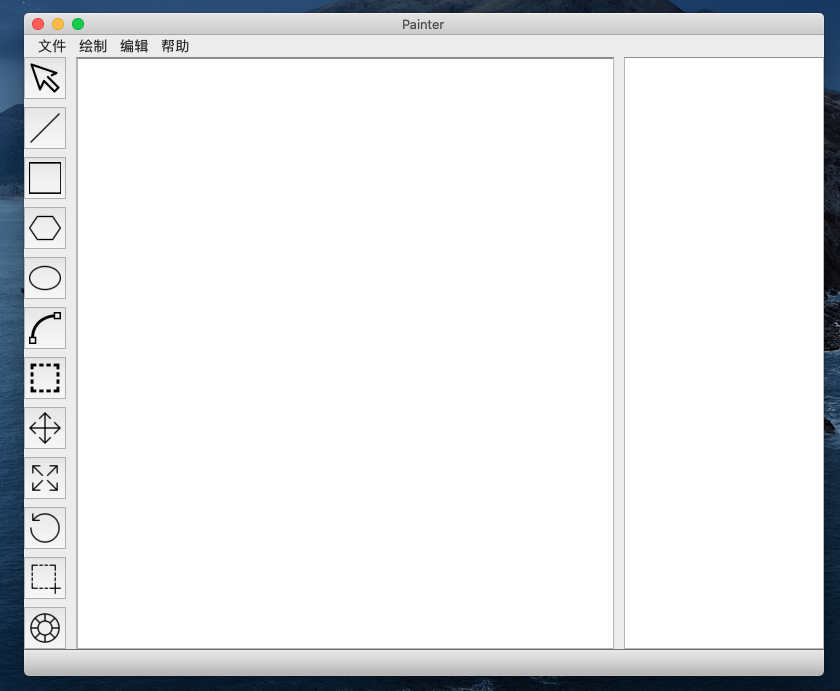
\includegraphics[scale=0.5]{Painter.png}
    \caption{Painter主界面}
\end{figure}

我们可以看到主界面可以一共分为三块:工具栏,画布和图元列表。

工具栏列出了一些常用的工具供用户使用,不必用户在菜单中选择,节省了用户的时间,也提高了易用性,而且每个工具上都有相应的简明图标的,而且当用户的鼠标移动到某一工具上时,还会自动提示该工具的功能。

画布是用户主要的绘制区域,该画布的大小可以由用户任意指定,而且可以在有限的显示区域内通过鼠标任意滑动到用户想要的区域。

图元列表会列出所有用户已经绘制的图元,并通过友好的命名来标识。

值得一提的是下面的状态栏,可以提示用户当前的状态,如上图中的就是"空闲",在绘制的状态时会提醒用户当前用什么算法在绘制什么图元。

\begin{figure}[H]
    \centering
    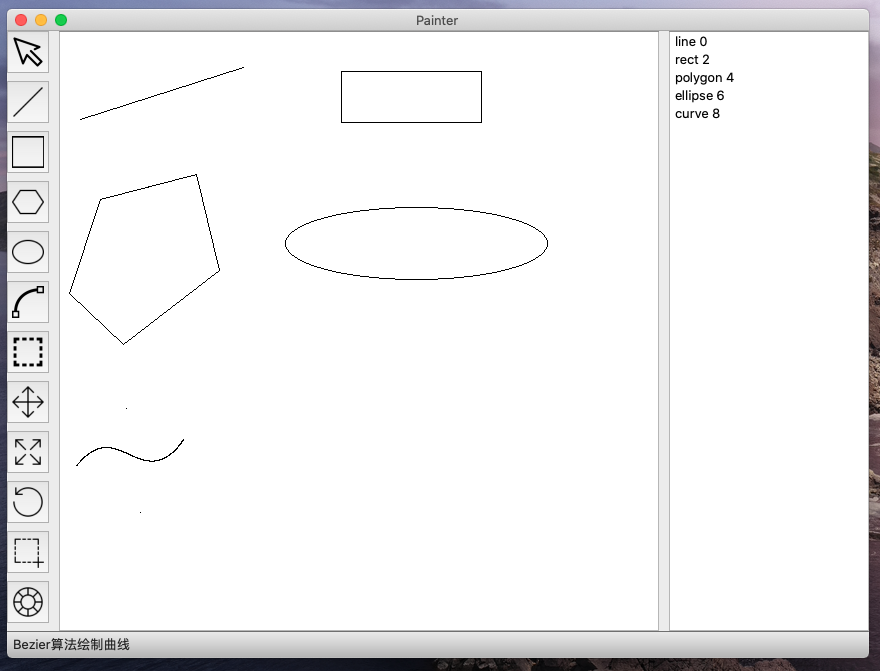
\includegraphics[scale=0.5]{Painting.png}
    \caption{Painter绘制中}
\end{figure}

\subsubsection{绘制功能}

绘制直线:点击直线图标,默认的算法是DDA算法,你也可以在菜单栏里选择别的算法。然后在canvas区域按下鼠标左键标记直线的起点,然后不要松开鼠标,一直拖动到你想设定的终点,你松开的那个点就是直线的终点,在移动鼠标的过程你可以看到直线是在一直动态变化的。

绘制矩形:点击矩形图标,跟直线的画法类似,先按下鼠标的左键,然后拖动再松开。 我这里采用PyQt的矩形绘制,其实用户也可以通过多边形绘制矩形,这里是为了方便用户而增加的一个绘制矩形的功能,因为是PyQt的矩形所以不能通过我的旋转算法进行旋转,缩放和平移是没有问题的。

绘制多边形:点击多边形的图标,这里跟直线的画法就不太一样了,因为多边形可以有任意多个点,而直线只有两个点。所以用户每按一次鼠标的左键就会产生一个新的控制点,因为多边形是封闭的,所以用户每次最后按下的点会和第一个点进行连线,用户双击鼠标就表示多边形绘制完成。

绘制椭圆:点击椭圆图标,这里的画法和直线和矩形的画法是一样的,其实将相当于画出一个矩形,然后在里面画一个椭圆。

绘制曲线:点击曲线图标,默认的算法是Bezier算法,你可以在菜单栏里选择别的算法。然后跟绘制多边形一样,每次鼠标左键点击都会产生一个控制点,最后双击鼠标,就表示曲线绘制完成。

\subsubsection{图元变换功能}

要变换图元的话,你需要先用选择工具选择要变换的图元,被选中的图元会被红色的框所包围,就如下图所示。

\begin{figure}[H]
    \centering
    
\includegraphics[scale=0.5]{select.png}
    \caption{选择图元}
\end{figure}

平移图元:平移图元的操作就是拖动,按下鼠标然后拖动,鼠标的相对位移就对应着图元的相对位移。所有的图元都可以进行平移操作。

缩放图元:先选择一个缩放的中心点,然后鼠标从另外的任意一个点开始拖动,开始拖动的点和中心点有一个向量,拖动中的点和中心点也有一个向量,这两个向量在x方向上的倍数(可以为负数)就是缩放系数。所有的图元都可以进行缩放操作。

旋转图元:跟缩放图元类似,先选择一个缩放的中心点,然后鼠标从另外的任意一个点开始拖动,开始拖动的点和中心点有一个向量,拖动中的点和中心点也有一个向量。这两个向量的旋转角就是图元的旋转角度。除了椭圆和矩形其他的图元都可以进行旋转操作。


\subsubsection{其他功能}

重置画布:用户可以重置画布并指定画布的大小:

\begin{figure}[H]
    \centering
    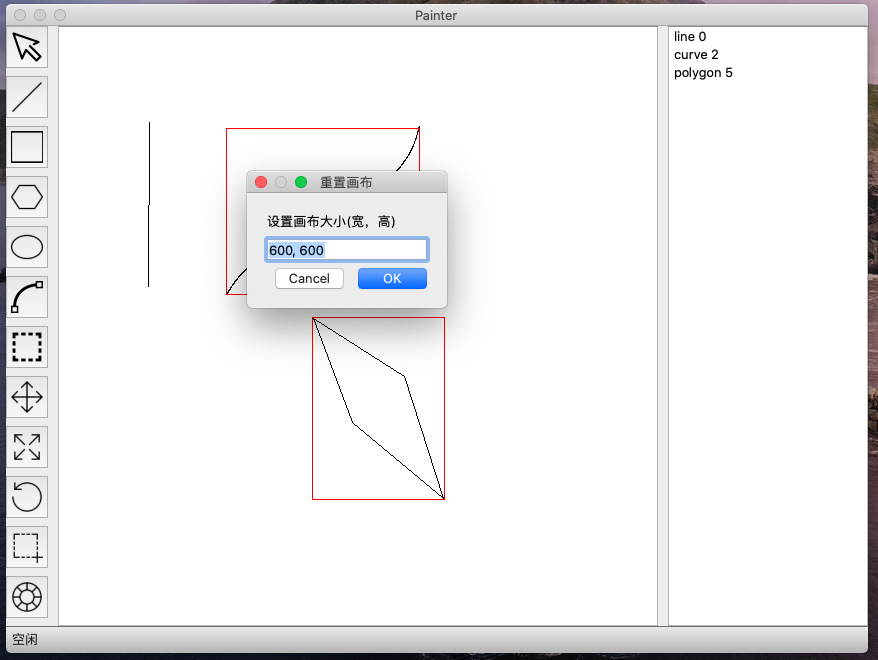
\includegraphics[scale=0.5]{reset.png}
    \caption{重置画布}
\end{figure}

设置画笔:用户可以通过调色板重新设置画笔的颜色,如下图,就设置了画笔为蓝色画了一个椭圆:

\begin{figure}[H]
    \centering
    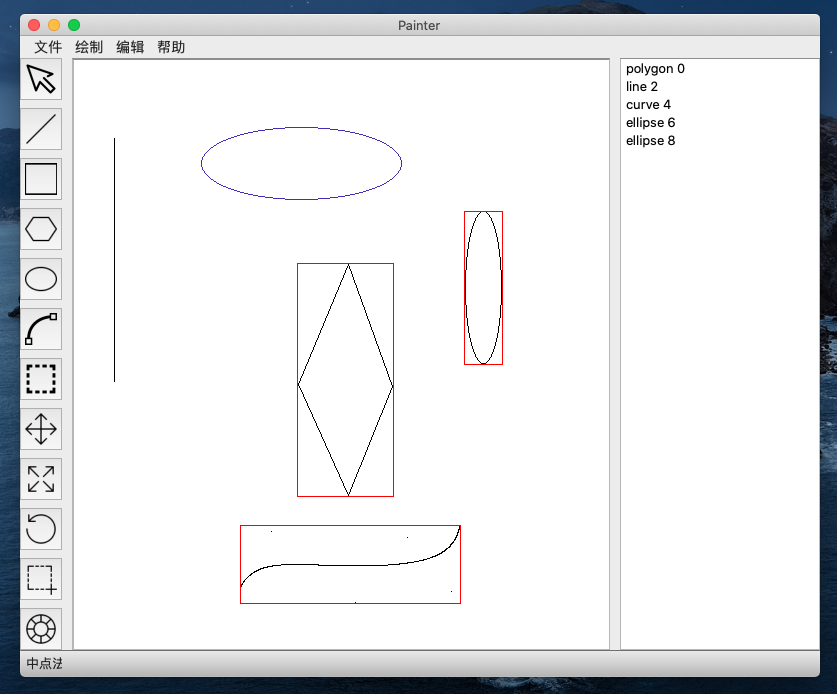
\includegraphics[scale=0.5]{color.png}
    \caption{设置画笔}
\end{figure}

保存文件:用户可以将自己的杰作保存成文件,支持png, jpg, bmp等格式,如下图我们就将刚刚的画作保存成了bmp文件:

\begin{figure}[H]
    \centering
    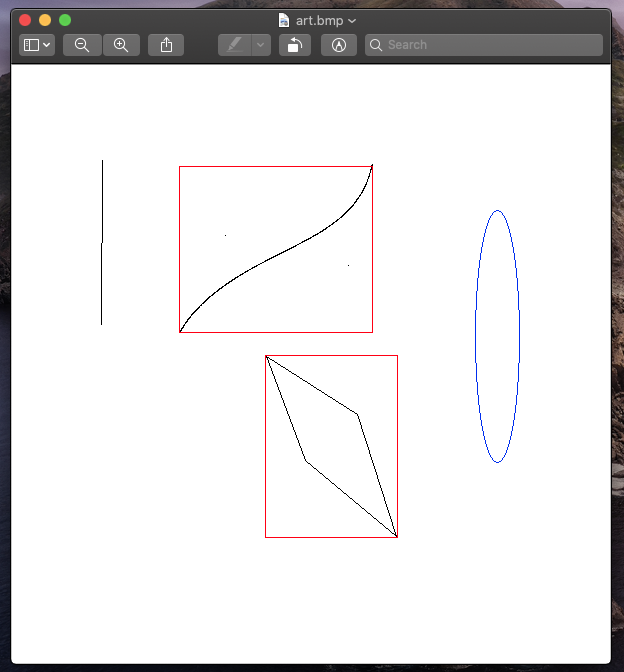
\includegraphics[scale=0.4]{save.png}
    \caption{保存文件}
\end{figure}


\section{总结}

这个项目实现了一些常见的图形学算法,并最终包装成一个完整的系统呈现出来。

\newpage

\bibliographystyle{plain}%
%"xxx" should be your citing file's name.
\bibliography{ref}

\end{document}